\section{The Kokkos Machine Model}\label{chap:kokkosMM}

The Kokkos machine model defines abstractions that represent hardware capabilities for processing and data access. The Kokkos parallel programming model exposes these abstractions to the programmer through C++ and the Kokkos API. By abstracting from physical hardware, the machine model ensures that applications written in programming models targeting this machine model are generic and performance-portable on current and future hardware. The Kokkos parallel programming model is one particular instance of a programming model that builds on top of that machine model. We would like to point out that it is this conceptual differentiation that allows scenarios where the underlying machine model is instantiated in other languages beyond C++, yet the algorithmic specification as well as performance characteristic and portability remain the same. 

The Kokkos abstract machine representation targets a design of a future shared-memory computing architectures. The design is shown in Figure~\ref{fig:spaces}. It is characterized by multiple latency-optimized execution units and off-die bandwidth-optimized accelerators. Both compute device types can have disjoint memory address spaces with unique performance properties. In such an architecture, execution units might be hierarchically organized with multiple levels of achievable parallelism with different memory access characteristics and coherence properties of caches. In order to ensure performance portability on such a wide range of configurations, an abstraction of compute resources and available memories are required. For this purpose we introduce the abstract concept called \emph{space}.

An instance of an \emph{execution space} is an abstraction over an execution resource to which a programmer can target parallel work. For example, an execution space can be used to describe a multi-core processor. In this case, the execution space contains several homogeneous cores organized into arbitrary logical groups. In a parallel programming model that implements this machine model, an instance of such an execution space would be made available to the programmer to run kernels. Adding more logical groups or accelerators simply increases the number of available execution spaces to the programmer.

Memory and memory types are exposed through \emph{memory spaces}. Each memory space provides storage capacity at which data structures can be allocated and accessed. Different memory space types have different characteristics with respect to accessibility from execution spaces and performance. 

An instance of a memory space provides a concrete method for the application programmer to request data storage allocations. Following the architecture as discussed earlier, the multi-core processor may contain multiple memory spaces that abstract on-package memory, slower DRAM and non-volatile memories. Accelerators can provide an additional memory space through its local on-package memory. This is also highligted in Figure~\ref{fig:spaces}. The programmer is free to decide where each data structure is allocated by requesting the corresponding memory space. Programmatically this is achieved by instantiating the according memory space. Kokkos provides the appropriate abstraction of memory allocation and data management. We believe that an abstract representation of execution- and memory devices is a key property towards performance-portable parallel programming.

How a machine model is exposed to the programmer and what the design considerations are towards defining an appropriate semantic capture are discussed in the next section.

%Ang, J.A., et. al., Abstract Machine Models and Proxy Architectures for Exascale Computing, 2014, Sandia National Laboratories and Lawrence Berkeley National Laboratory, DOE Computer Architecture Laboratories Project

\begin{figure}

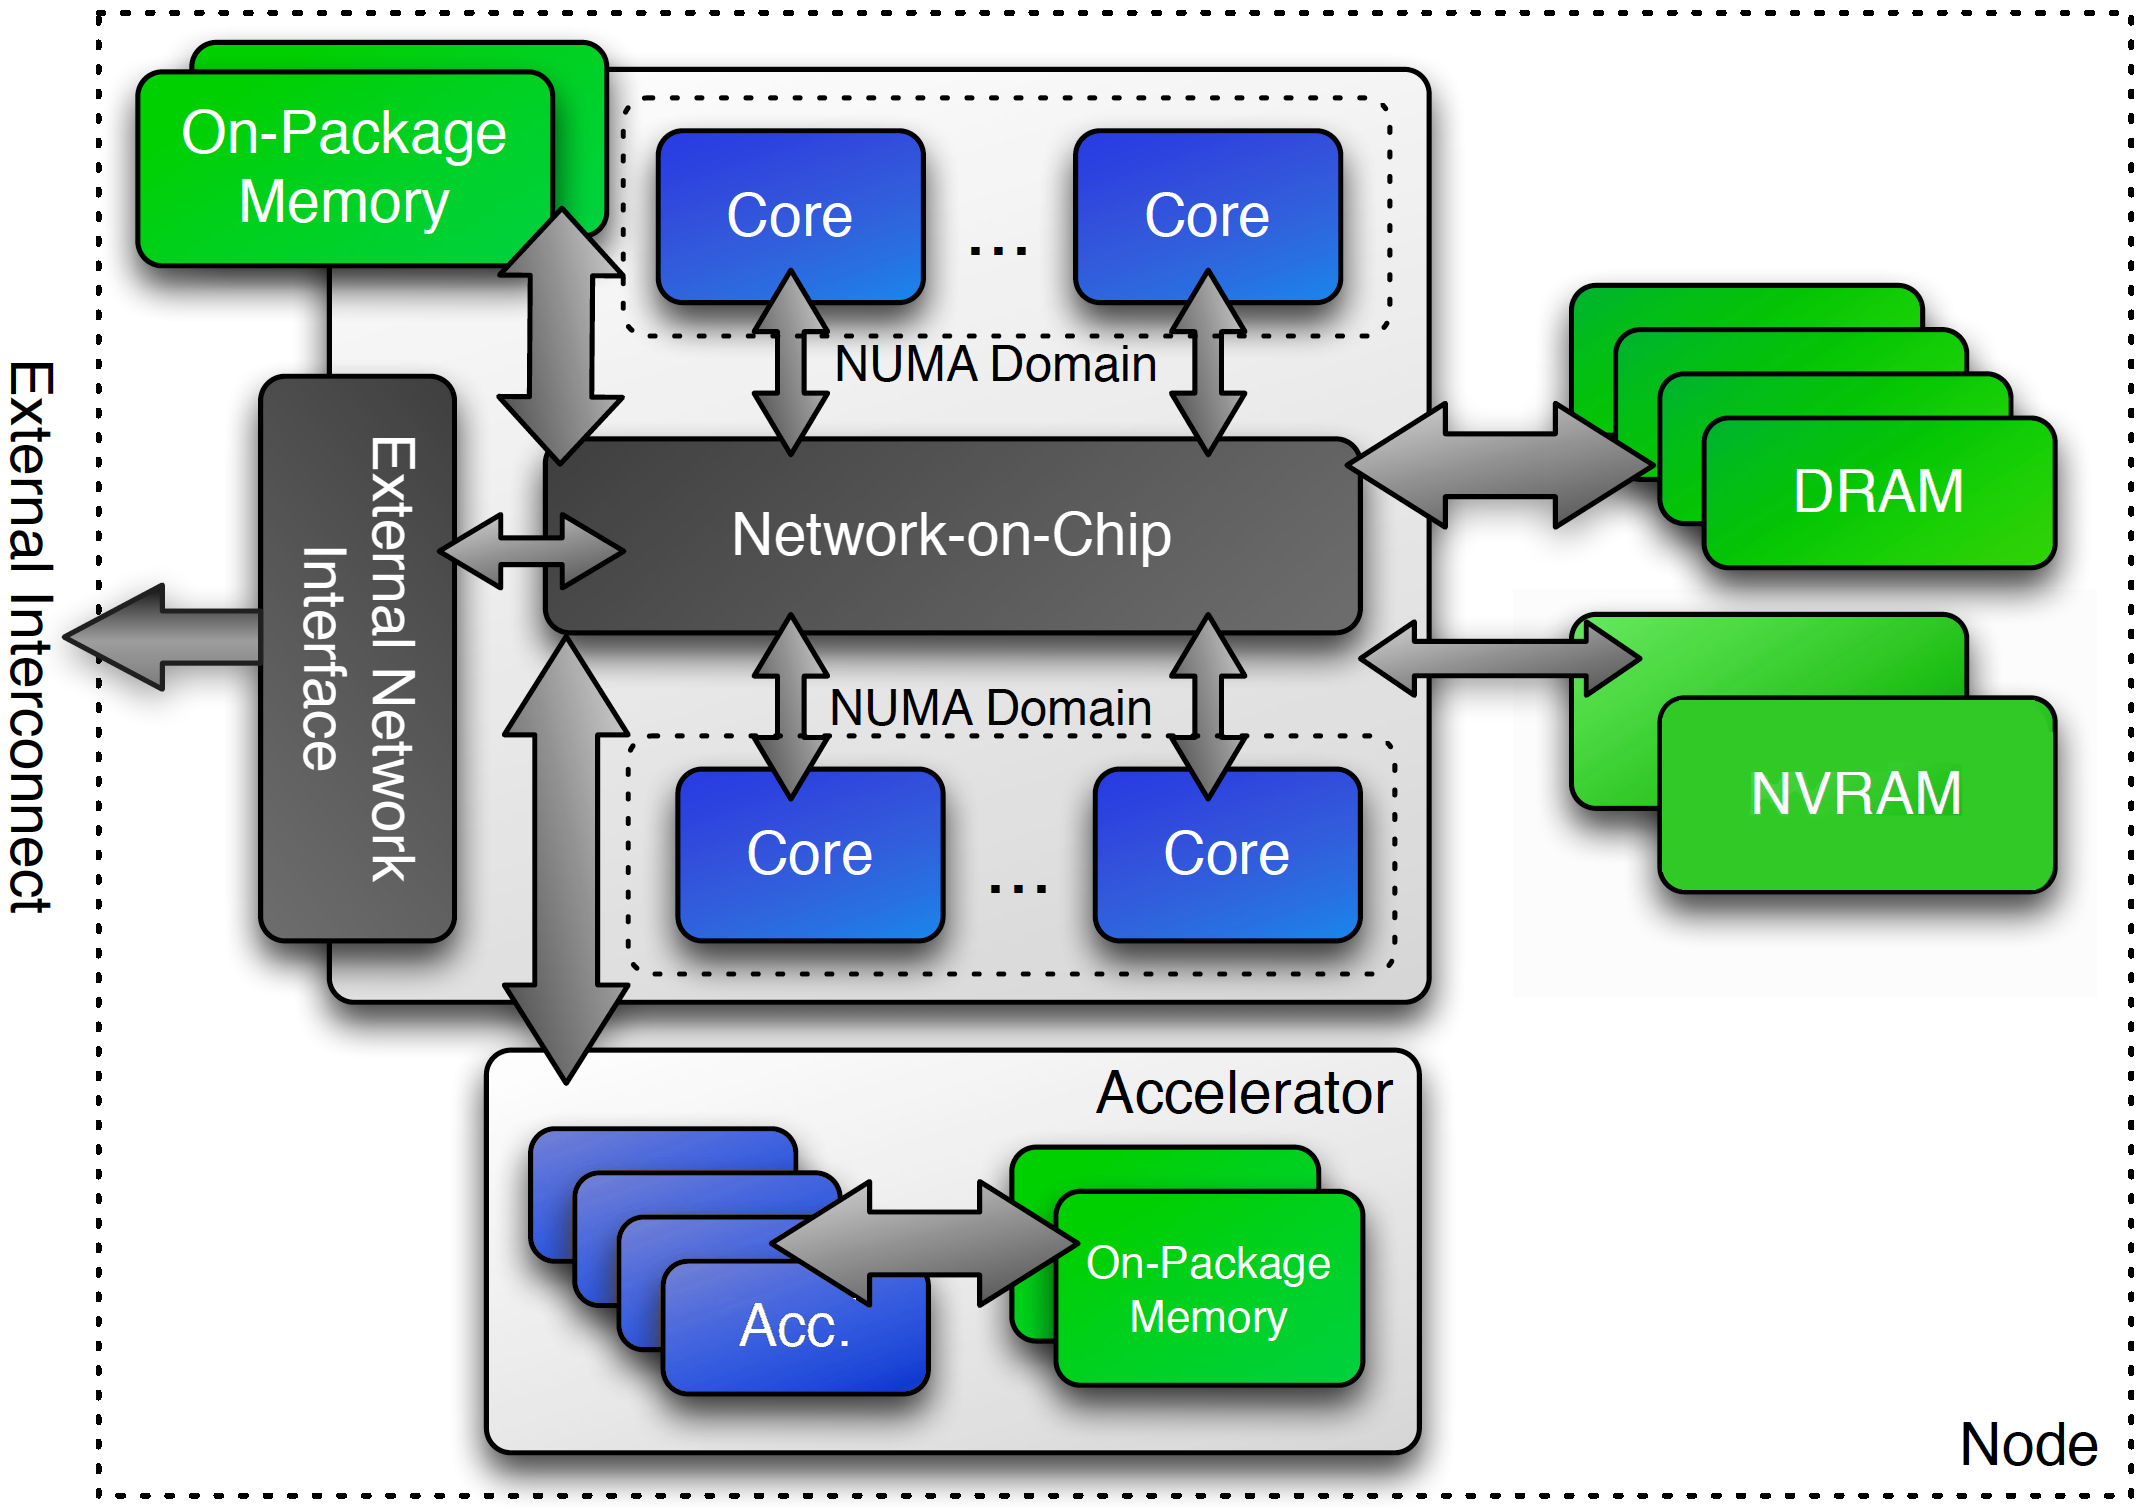
\includegraphics[width=0.5\textwidth]{img/KokkosSpaces.png}
\caption{Spaces represent conceptual building blocks of the abstract machine model in Kokkos.}
\label{fig:execspace}
\label{fig:spaces}
\end{figure}
